\begin{figure}
  \centering
  Full Gramian\\
  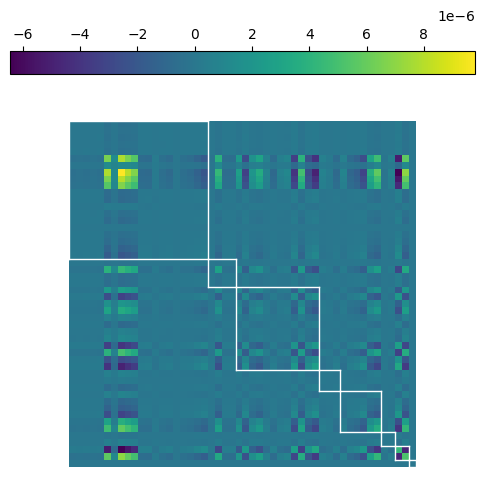
\includegraphics[width=0.43\linewidth]{../kfac_pinns_exp/exp04_gramian_contributions/fig/gram_full.png}

  \begin{tabular}{ccc}
    (forward, forward)
    &
      (forward, gradient)
    &
      (forward, Hessian)
    \\
    
\includegraphics[width=0.33\linewidth]{../kfac_pinns_exp/exp04_gramian_contributions/fig/gram_output_output.png}
    &
      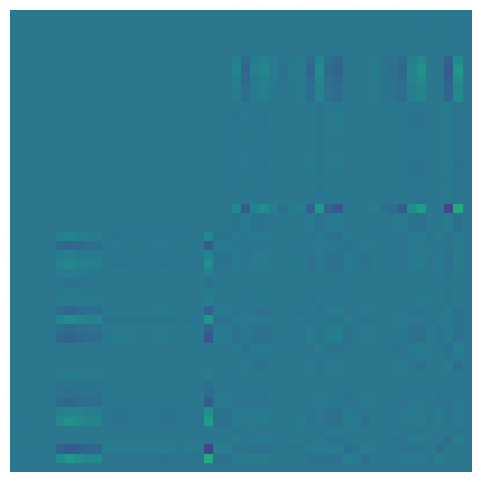
\includegraphics[width=0.33\linewidth]{../kfac_pinns_exp/exp04_gramian_contributions/fig/gram_output_grad_input.png}
    &
      
\includegraphics[width=0.33\linewidth]{../kfac_pinns_exp/exp04_gramian_contributions/fig/gram_output_hess_input.png}
    \\
    &
      (gradient, gradient)
    &
      (gradient, Hessian)
    \\
    &
      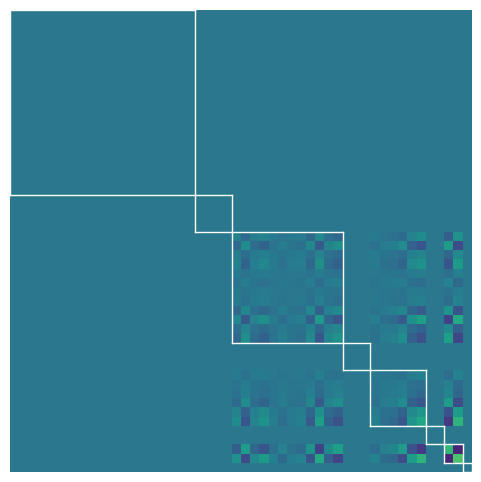
\includegraphics[width=0.33\linewidth]{../kfac_pinns_exp/exp04_gramian_contributions/fig/gram_grad_input_grad_input.png}
    &
      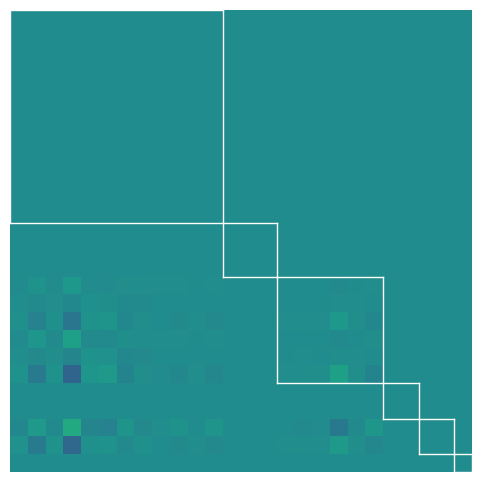
\includegraphics[width=0.33\linewidth]{../kfac_pinns_exp/exp04_gramian_contributions/fig/gram_grad_input_hess_input.png}
    \\
    &
    &
      (Hessian, Hessian)
    \\
    &
    &
      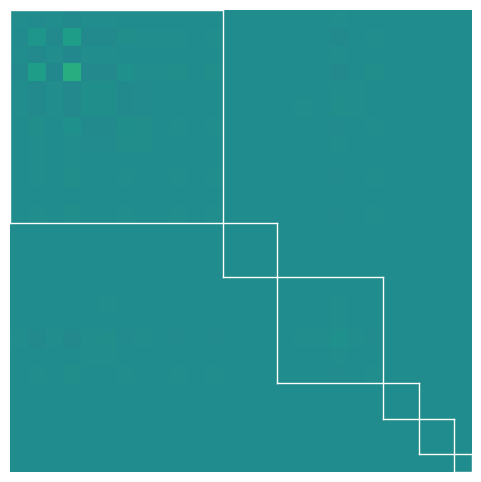
\includegraphics[width=0.33\linewidth]{../kfac_pinns_exp/exp04_gramian_contributions/fig/gram_hess_input_hess_input.png}
  \end{tabular}
  \caption{Contributions to the Gramian from different children in the
    computation graph.}\label{fig:gramian-contribution-children}
\end{figure}
%%% Local Variables:
%%% mode: latex
%%% TeX-master: "../main"
%%% End:
